\begin{figure}[t]
    \centering
\textbf{}    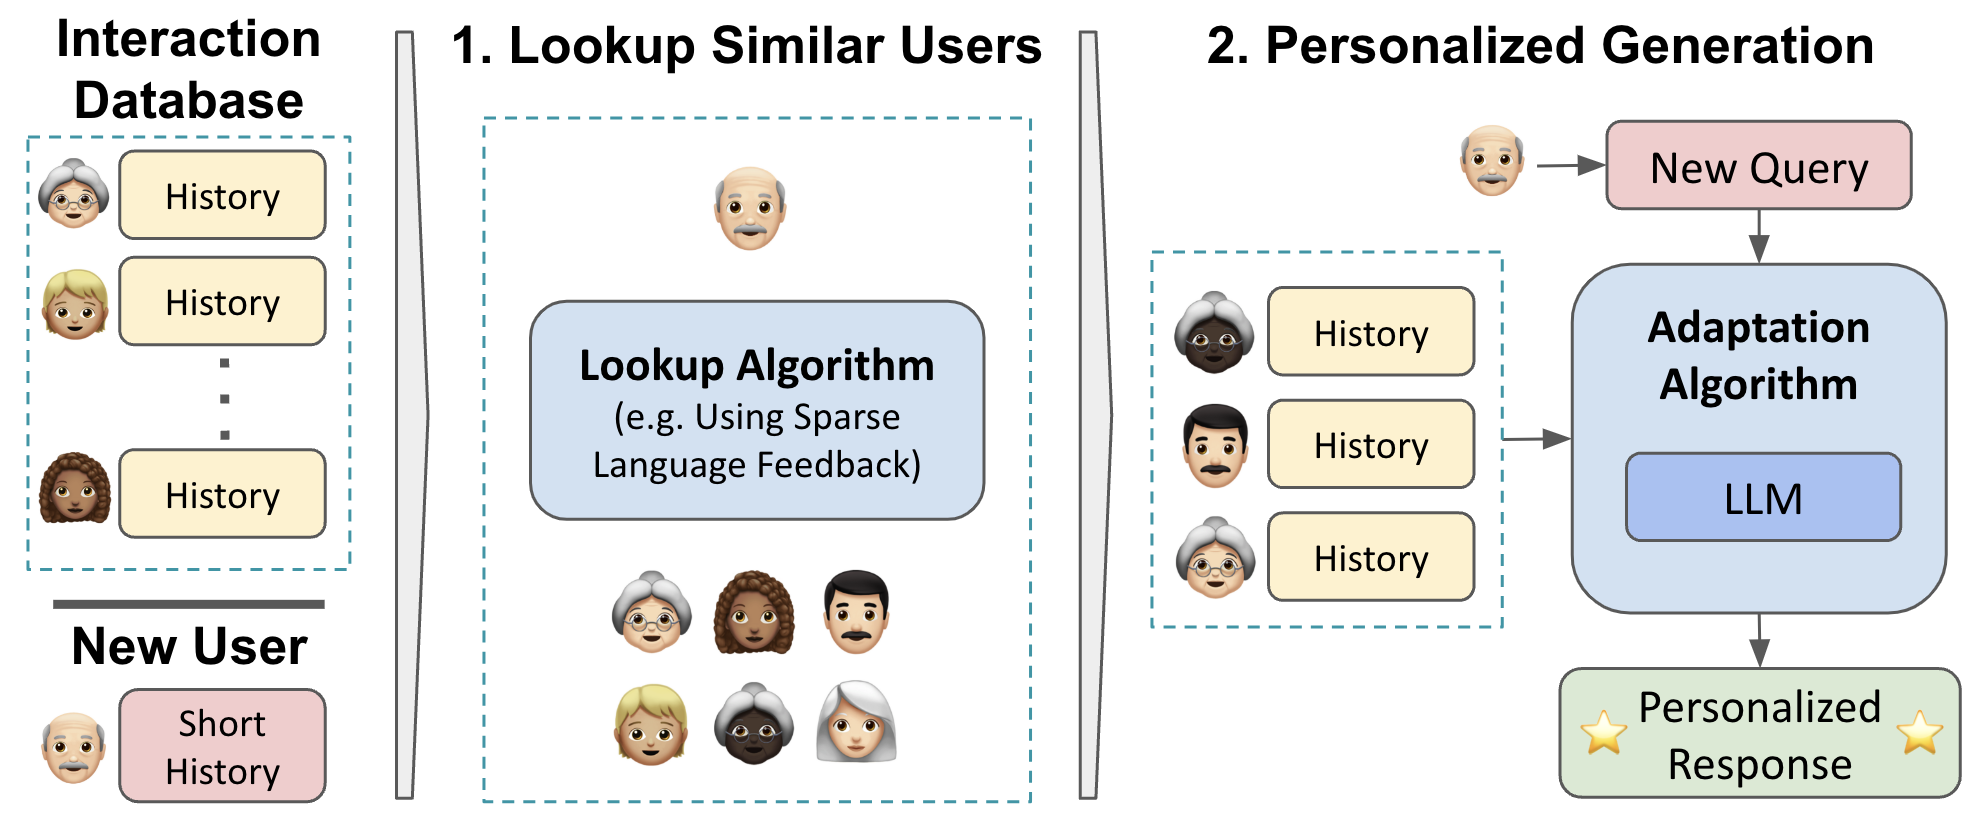
\includegraphics[width = \textwidth]{figures/metalearn_fig.png}
    \caption{In the canonical personalization setting, a dataset of historical users and their interactions is leveraged to personalize interactions for a new user with a limited history. \textsf{PersonalLLM} enables the development of such methods for learning \textit{across} users.}
    \label{fig:metalearn}
\end{figure}

\section{PersonalLLM}\label{sec:dataset}

Our \textsf{PersonalLLM} testbed is composed of two high-level components:
1) a dataset of prompts, each paired with a set of high-quality responses among which humans would be expected to display diverse preferences and
2) a method for sampling diverse personal preference models, such that we can test methods for personalization using these ``personas'' as our simulated users.
Next, we will describe each of them in detail.  Our data \footnote{\url{https://huggingface.co/datasets/namkoong-lab/PersonalLLM}} and code \footnote{\url{https://github.com/namkoong-lab/PersonalLLM}} are publicly available,  and full documentation for our dataset is available in Appendix~\ref{app:add_data_det}.

\begin{figure}[t]
    \centering
    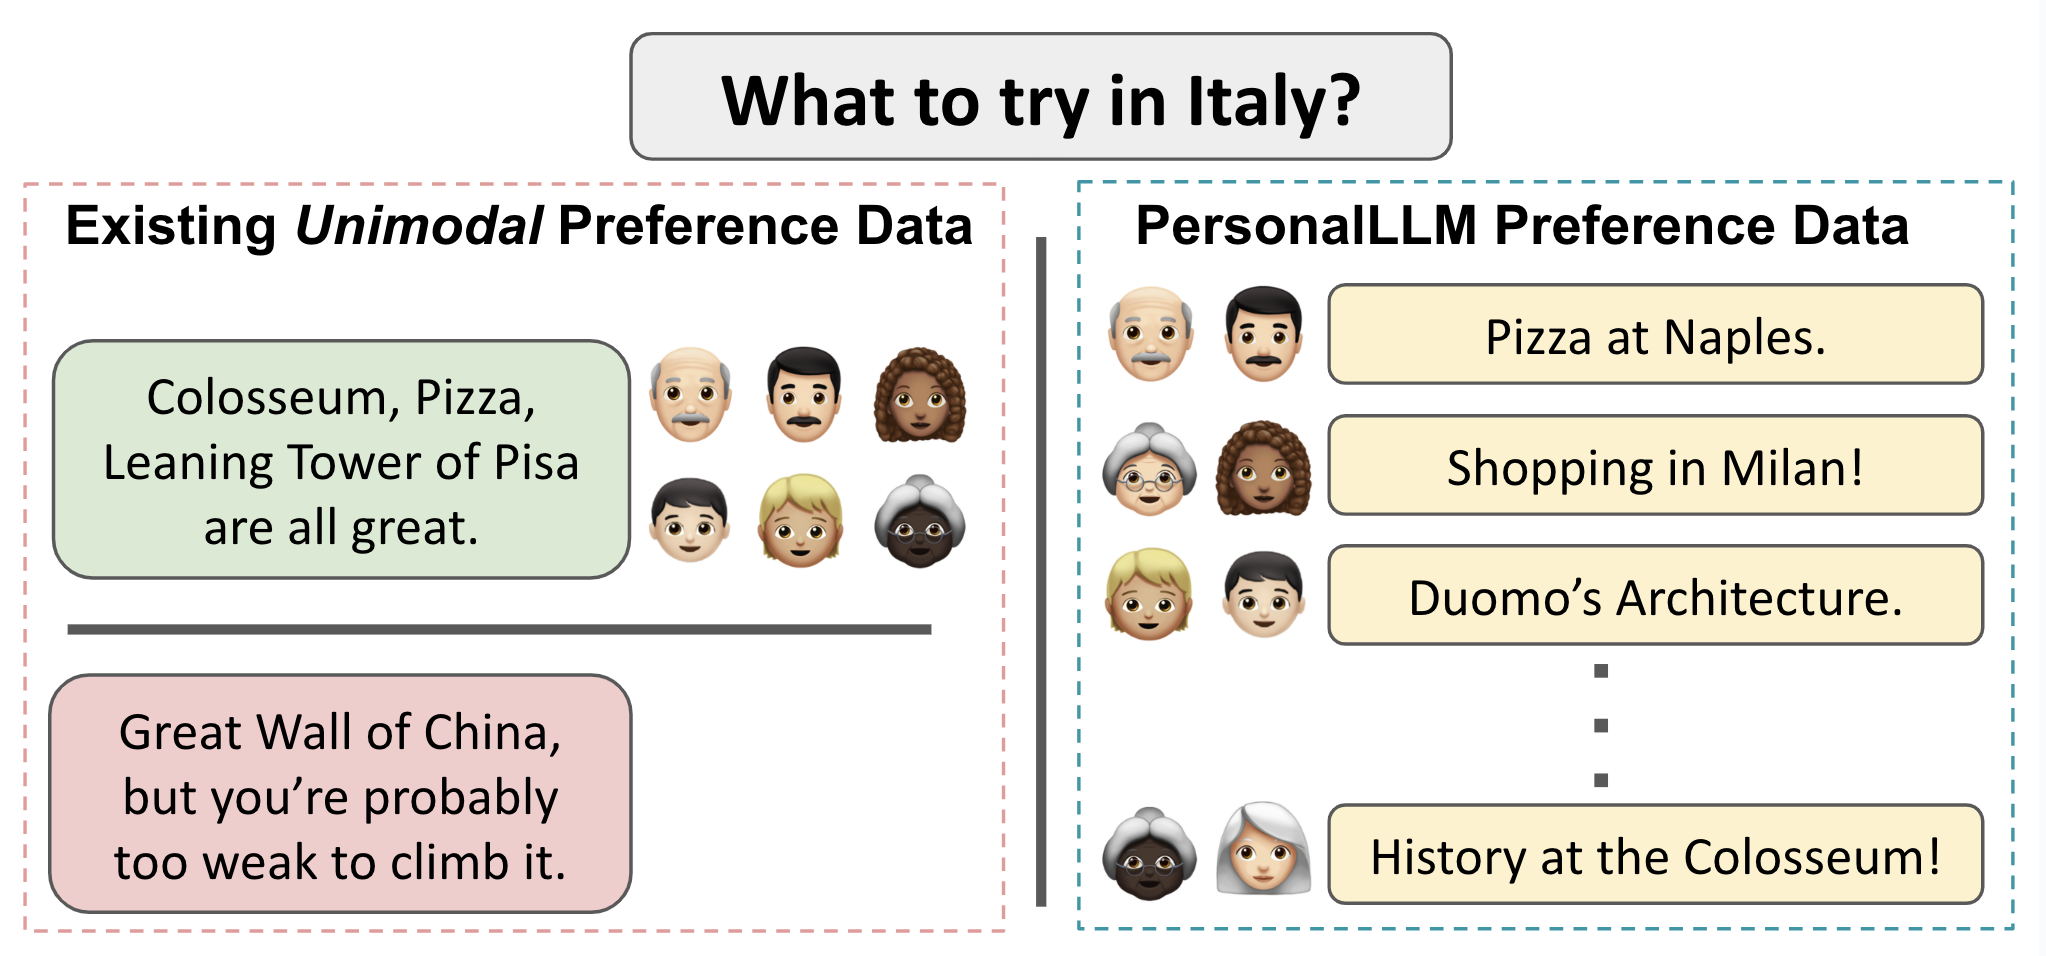
\includegraphics[width = \textwidth]{figures/data_example.png}
    \caption{\textbf{Left:} Existing alignment datasets contain prompts paired with multiple responses, where the majority of people are expected to prefer one specific response (e.g., a harmless response). \textbf{Right:} Our dataset consists of prompts paired with many high-quality responses, each favored by different personas. Such a dataset induces diverse preferences in our personal preference models, creating a testbed to build \textsf{PersonalLLM}s.}
    \label{fig:PersonalLLM}
\end{figure}

\subsection{Dataset}

Since our goal is to study diverse preferences, we first focus on collecting \textit{open-ended} prompts, similar to a chat setting.
We compile 37,919 prompts from Anthropic Helpful-online, Anthropic Helpful-base \citep{bai2022training}, Nvidia Helpsteer \citep{wang2023helpsteermultiattributehelpfulnessdataset}, and RewardBench \citep{lambert2024rewardbench}.
From this set, prompts are filtered to those with a length of 2400 characters or fewer as most reward models are limited to 4096 context length. We then randomly draw 10,402 prompts to form our final set.

Our next aim is to collect many high-quality responses for each prompt. 
Important desiderata for the generated responses are that i) they do not exhibit much variation in terms of undesirable contents (like misinformation or toxicity) or obvious dimensions of helpfulness or length, as is typical in RLHF datasets, ii) they exhibit diversity across meaningful dimensions of personal preferences like political viewpoint and culture, as well as difficult to describe latent features.
To achieve this, we generate eight responses for each of these 10,402 prompts using a selection of the top models from ChatArena and other important benchmarks: \textbf{ GPT-4o, Claude 3 Opus, Gemini-Pro-1.5, Command-R-Plus, GPT-4-Turbo, Claude 3 Sonnet, Llama3-70B-Instruct, and Mixtral 8x22B}. We split the resulting dataset into 9,402 training examples and 1,000 test examples. 

\subsection{Simulating Personal Preference Models}\label{sec:sim_users}

We design our approach to creating simulated \textsf{PersonalLLM} users with several goals in mind.
First, we aim for \textsf{PersonalLLM} to allow for the simulation of a large number of users, enabling the study of the full personalization paradigm for applications such as search engines and recommender systems \citep{davidson2010youtube, das2007google, Xu_2022, F_rber_2020} wherein a historical database of user data is leveraged to personalize new interactions.
Next, when applied to our dataset, our preference models should allow for the study of alignment based on diverse and complex latent preferences, as opposed to simple attributes such as answer length or sensitive and reductive user characteristics, for example, race or gender.
Finally, our evaluation should not rely on GPT4, which can be expensive and unsuitable for research purposes given model opacity and drift.
While human evaluation like that of \citet{kirk2024prismalignmentprojectparticipatory} is a gold standard, wherein 
fine-grained preference feedback is gathered from a representative sample of diverse and multicultural participants, it is impractical or even impossible to get this feedback throughout the methodology development cycle, meaning that synthetic personal preference models will ultimately be needed.

To overcome this difficult challenge of simulating diverse preferences, we propose a solution based on a set of strong open-source RLHF reward models.  
While it may be the case that different reward models have fairly uniform preferences over the high-quality/low-quality response pairs on which they are typically trained, we hypothesize that their preferences over many high-quality responses will instead be diverse.

Since the number of existing top-quality reward models is much smaller than the number of users we would like to simulate, we propose to generate users by sampling weightings over the set of reward models, such that the reward score assigned to a (prompt, response) pair by a user is a weighted sum of the reward scores assigned by the pre-trained reward models.
In Section~\ref{sec:persona_analysis}, we validate our hypothesis regarding the diverse and non-trivial preferences created by such sampling.

More formally, for an input prompt $x \in \mathcal{X}$, an LLM produces output response $y \in \mathcal{Y}$, where $\mathcal{X}$ and $\mathcal{Y}$ are the set of all-natural language.  Then, a preference model $\text{R}: \mathcal{X} \times \mathcal{Y} \rightarrow \mathbb{R}$ assigns a reward score to the response given to the prompt, with higher scores indicating better responses.  
Next, consider a set of $B$ base reward models, denoted as $\text{RM}_b$, $b=1,\dots,B$, and a set of $k$ $B$-\text{dimensional} weightings, which represent a set of personal preference models.  
The preference model corresponding to user $i$ can then be defined by a weighted average of these $B$ base models $\text{RM}_1, \text{RM}_2,\dots, \text{RM}_{B}$, with weights $w_1, w_2,\dots, w_B$:
\begin{align}
\vspace{-3pt}
    \text{R}^i(x,y) = \sum_{b=1}^{B} w^i_{b}\cdot\text{RM}_b(x,y)
\vspace{-3pt}
\end{align}
For our base reward models $\{\text{RM}_b\}_{b=1}^B$, we select 10 reward models with strong performance on RewardBench, an open-source benchmark for evaluating reward models.  
These reward models are built on top of popular base models such as Llama3, Mistral, and Gemma (see Appendix~\ref{app:add_data_det}).  
We evaluate each (prompt, response) pair in the train and test set with each model so that for any personality created in this manner, each (prompt, response) pair in the dataset can be scored via a simple weighting.

Taken together, our dataset and personal preference models provide an innovative and challenging environment in which to develop personalization methodology, extending the existing paradigm of simulated rewards for domains like recommender systems \citep{zhao2023kuaisimcomprehensivesimulatorrecommender, ie2019recsimconfigurablesimulationplatform} to the task of LLM personalization.

\subsubsection{Sampling User Weightings}
There are many valid ways to sample the $B$-dimensional weighting vectors.  As a simple starting point, we propose to sample from a Dirichlet distribution with a uniform concentration parameter across all classes ($w \sim \text{Dirichlet}(\alpha)$).  
As $\alpha$ becomes very small, the preference models converge towards the 10 base reward models; as it becomes large, preferences become unimodal.  Such a parameter allows us to simulate user bases with different underlying preference structures, as we detail in the next section.



